\documentclass{article}
%packages
\usepackage{graphicx}
\usepackage[latin1]{inputenc}
\usepackage[T1]{fontenc}
\usepackage[frenchb]{babel}
\usepackage[a4paper]{geometry}
\usepackage{textcomp}
\begin{document}
%title
\begin{titlepage}
	\vspace{-20px}
	\begin{tabular}{l}
    \textsc{Blin} S\'ebastien\\
    \textsc{Collin} Pierre-Henri\\
    \textsc{Eula} Florian
	\end{tabular}
	\hfill \vspace{10px}
\includegraphics[scale=0.1]{esir.png}\\
	\vfill
	\begin{center}
    \Huge{\'Ecole sup\'erieure d'ing\'enieurs de Rennes}\\
    \vspace{1cm}
    \LARGE{1\`ere Ann\'ee}\\
    \large{Parcours Informatique}\\
    \vspace{0.5cm}\hrule\vspace{0.5cm}
    \LARGE{\textbf{ARC2}}\\
    \Large{Compte-Rendu TP \no 2}
    \vspace{0.5cm}\hrule
    \vfill
    \vfill
	\end{center}
	\begin{flushleft}
    \Large{Sous l'encadrement de~:}\\
    \vspace{0.2cm}
    \large{{Christophe} Wolinski}
	\end{flushleft}
	\vfill
\end{titlepage}
\section{Interface d'entr\'ees/sorties avec test d'\'etat}
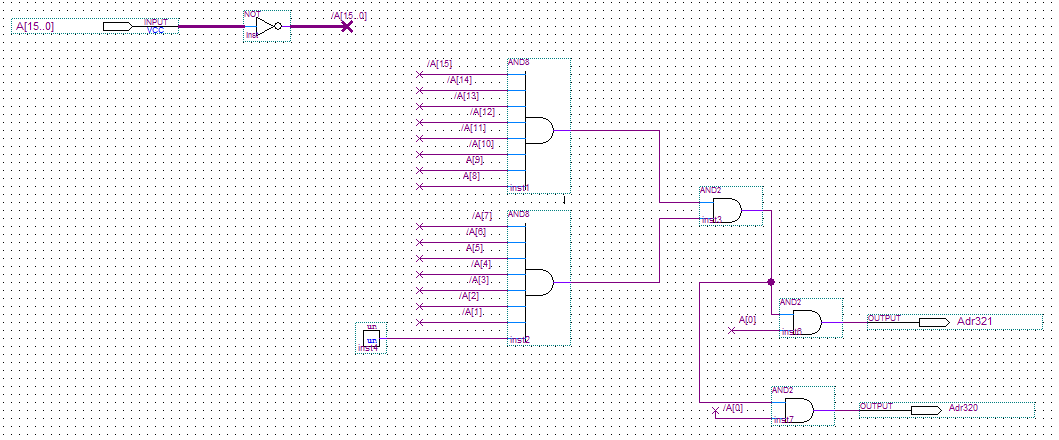
\includegraphics[scale=0.5]{selecteur.PNG}\\
Le sch\'ema ci-dessus permet de s\'electionner l'adresse 320h ou 321h.\\
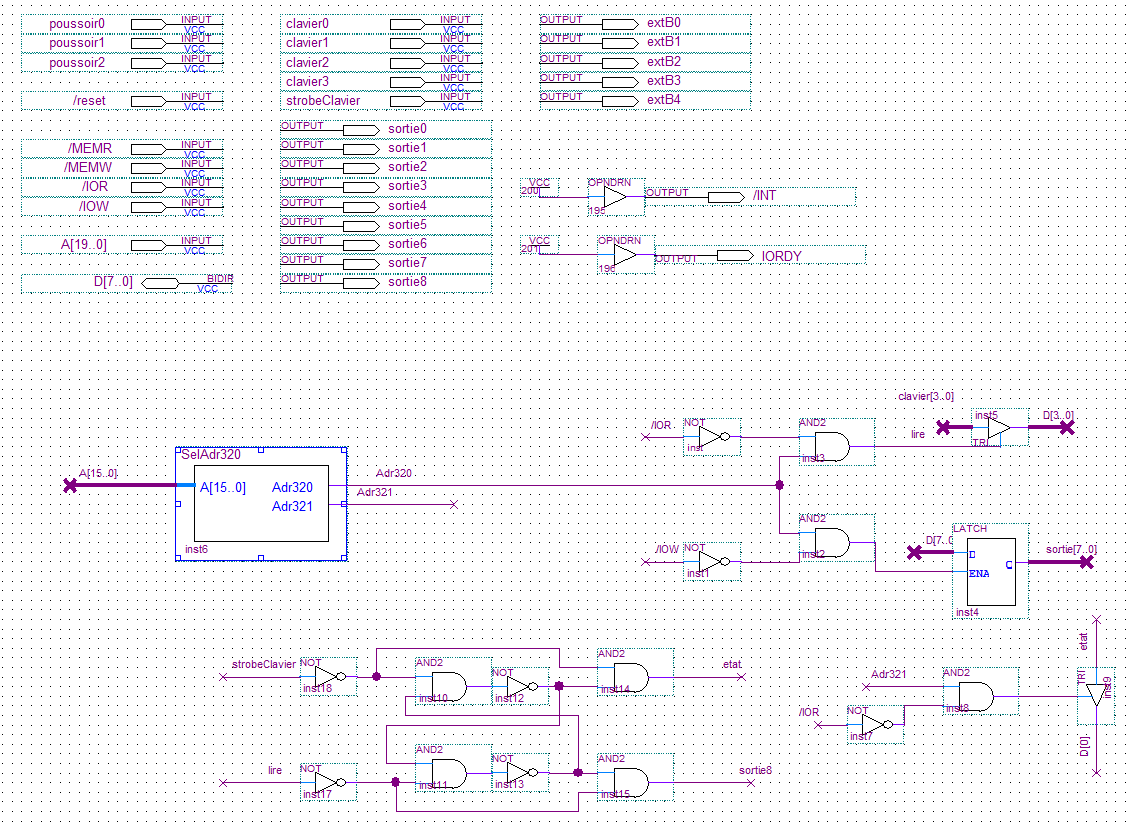
\includegraphics[scale=0.5]{fpga111.PNG}\\
La sortie Adr320 de SelAdr320 et l'entr\'ee IOR permettent de lire la valeur du clavier (l'entr\'ee clavier[3..0]).\\
La sortie Adr321 de SelAdr320 et l'entr\'ee IOR permettent de lire la valeur de l'\'etat.\\
Le verrou RS emp\^eche d'envoyer des flux de donn\'ees pendant l'appui d'un bouton sur le clavier.
\section{Lecture d'une donn\'ee avec test d'\'etat}
\begin{verbatim}
.model small
.data
.stack
.code

.start:
    MOV	ax,@
    MOV	ds,ax           ;initialisation de DS
somme:
    CALL	LIRE_CLAVIER
    MOV	BL, AL
    CMP AL, 0
    JZ fin
    CALL	LIRE_CLAVIER
    ADD	BL, AL          ;somme des deux chiffres
    CMP AL, 0
    JNZ	somme
fin:
    MOV AL, BL
    MOV	DX,	0320H
    OUT	DX,	AL
    MOV	AH,	4CH
    INT	21H
    
;;;;;Procedure lire clavier
lire_clavier:
    PUSH BP
    MOV	 BP,SP
Boucle:	
    MOV	DX,321h
    IN	AL,DX
    AND	AL,00000001b
    JZ	Boucle
    MOV	DX,320h
    IN	AL,DX
    POP    BP
    RET

END
\end{verbatim}
\end{document}

